\documentclass[a4paper, 12pt]{article}

%Абзацный отступ

\usepackage{indentfirst}

%Рисунки

\usepackage{subfig}
\usepackage{graphicx}
\usepackage{wrapfig}

%Гиперссылки и работа с цветом

\usepackage{hyperref}
\usepackage[rgb]{xcolor}
\hypersetup{			%Гиперссылки
	colorlinks=true, 	%false: ссылки в рамках
	urlcolor=blue		%на URL
}

%Русский язык

\usepackage[T2A]{fontenc}		%кодировка
\usepackage[utf8]{inputenc}		%кодировка исходного текста
\usepackage[english, russian]{babel}	%локализация и переносы


%Математика

\usepackage{amsmath, amsfonts, amssymb, amsthm, mathtools, mathrsfs}

%Пакет с градусом

\usepackage{gensymb}

\author{Штрайх Роберт}
\title{Работа 3.6.1. Спектральный анализ электрических сигналов}
\date{21 ноября 2021 г.}

\begin{document}
\begin{titlepage}
	\centering
	\vspace{5cm}
	{\scshape\LARGE Московский физико-технический институт \par}
	\vspace{4cm}
	{\scshape\Large Лабораторная работа №3.6.1 \par}
	\vspace{1cm}
	{\huge\bfseries Спектральный анализ электрических сигналов\par}
	\vspace{1cm}
	\vfill
\begin{flushright}
	{\Large выполнил студент 006 группы ФЭФМ}\par
	\vspace{0.3cm}
	{\Large Штрайх Роберт}
\end{flushright}
	

	\vfill

% Bottom of the page
	Долгопрудный, 2021 г.
\end{titlepage}

\newpage

\textbf{Цель работы:} изучить спектры электрических сигналов.

\textbf{В работе используются:} генератор сигналов произвольной формы, цифровой осциллограф с функцией быстрого преобразования Фурье.

\section{Теоретическое введение}
\subsection*{Разложение сложных сигналов на периодические колебания}

Метод для описания сигналов. Для него используется разложение в сумму синусов и косинусов с различными аргументами или, как чаще его называют, \textit{разложение в ряд Фурье}.

Пусть задана функция $f(t)$, которая периодически повторяется с частотой $\Omega_1 = \dfrac{2\pi}{T}$, где $T$ --- период повторения импульсов. Её разложение в ряд Фурье имеет вид 
\begin{equation}
f(t) = \dfrac{a_0}{2} + \sum\limits_{n = 1}^{\infty}\left[a_n \cos \left(n \Omega_1t\right) + b_n \sin \left(n \Omega_1t\right)\right]
\end{equation}
или
\begin{equation}
f(t) = \dfrac{a_0}{2} + \sum\limits_{n = 1}^{\infty}A_n \cos \left(n\Omega_1t-\psi_n\right)
\end{equation}
Если сигнал четен относительно $t=0$, так что $f(t) = f(-t)$ в тригонометрической записи остаются только косинусные члены. Для нечетной наоборот.

Коэффициенты определяются по формуле
\begin{equation}
\begin{array}{c}
a_n  = \dfrac{2}{T}\int\limits_{t_1}^{t_1+T}f(t)\cos\left(n \Omega_1 t\right) dt\\
\\
b_n = \dfrac{2}{T}\int\limits_{t_1}^{t_1+T}f(t)\sin\left(n \Omega_1 t\right) dt
\end{array}
\end{equation}
Здесь $t_1$ --- время, с которого мы начинаем отсчет.

Сравнив формулы $(1)$ и $(2)$ можно получить выражения для $A_n$  и $\psi_n$:
\begin{equation}
A_n = \sqrt{a_n^2+b_n^2};\psi_n = \arctan \dfrac{b_n}{a_n}
\end{equation}

\subsection*{Периодическая последовательность прямоугольных импульсов}

Введем некоторые величины:
\[\Omega_1 = \dfrac{2\pi}{T}, \]
где $T$ --- период повторения импульсов.

Коэффициенты при косинусных составляющих будут равны
\begin{equation}
a_n = \dfrac{2}{T}\int\limits_{-\tau/2}^{\tau/2}V_0\cos\left(n\Omega_1 t\right)dt = 2V_0\dfrac{\tau}{T}\dfrac{\sin\left(n\Omega_1\tau/2\right)}{n\Omega_1\tau/2} \sim \dfrac{\sin x}{x}
\end{equation}

Здесь $V_0$ - амплитуда сигнала.

Поскольку наша функция четная, то $b_n = 0$. 

Пусть у нас $\tau$ кратно $T$. Тогда введем ширину спектра, равную $\Delta \omega$ --- расстояние от главного максимума до первого нуля огибающей, возникающего, как нетрудно убедится при $n = \dfrac{2\pi}{\tau \Omega_1}$. При 
этом
\begin{equation}
\label{delta nu*t}
\Delta \omega \tau \simeq 2\pi \Rightarrow \Delta \nu \Delta t \simeq 1
\end{equation}

\subsection*{Периодическая последовательность цугов}
Функция $f(t)$ снова является четной относительно $t = 0$. Коэффициент при $n$-ой гармонике согласно формуле $(3)$ равен
\begin{equation}
a_n = \dfrac{2}{T}\int\limits_{-\tau/2}^{\tau/2}V_0 \cos \left(\omega_0t\right) \cdot \cos\left(n \Omega_1t\right)dt = V_0 \dfrac{\tau}{T}\left( \dfrac{\sin\left[\left(\omega_0 - n \Omega_1\right)\dfrac{\tau}{2}\right]}{\left( \omega_0 - n \Omega_1\right) \dfrac{\tau}{2}} + \dfrac{\sin\left[\left(\omega_0 + n \Omega_1\right)\dfrac{\tau}{2}\right]}{\left( \omega_0 + n \Omega_1\right) \dfrac{\tau}{2}}\right)
\end{equation}

\subsection*{Амплитудно-модулированные колебания}
Рассмотрим гармонические колебания высокой частоты $\omega_0$, амплитуда которых медленно меняется по гармоническому закону с частотой $\Omega \ll \omega_0$.
\begin{equation}
f(t) = A_0 \left[1+m\cos \Omega t\right] \cos \omega_0 t
\end{equation}
Коэффициентом $m$ называется \textit{глубина модуляции}. При $m < 1$ амплитуда меняется от минимальной $A_{min} = A_0(1-m)$ до максимальной
 
$A_{max} = A_0(1+m)$. Глубина модуляции может быть представлена в виде
\begin{equation}
m = \dfrac{A_{max}-A_{min}}{A_{max}+A_{min}}
\end{equation}
Простым тригонометрическим преобразованием уравнения $(9)$ можно найти спектр колебаний
\begin{equation}
f(t) = A_0 \cos \omega_0t + \dfrac{A_0m}{2} \cos \left(\omega_0 + \Omega\right)t + \dfrac{A_0m}{2}\cos\left(\omega_0 - \Omega\right)t
\end{equation}

\section{Ход работы}
\subsection*{Исследование спектра периодической последовательности прямоугольных импульсов}

Устанавливаем прямоугольные колебания с $f_\text{повт}$ = 1 кГц и длительностью импульса $\tau$ = 100 мкс.

Получаем спектр сигнала и, изменяя либо $\tau$, либо $f_\text{повт}$, наблюдаем, как он изменяется.

Ширина спектра $\Delta \nu$ в случае изменения $f_\text{повт}$ от 1 кГц до 2 кГц не изменилась, но уменьшилась при повышении $\tau$. $\delta \nu$ увеличилась при повышении $f_\text{повт}$.

Проведем измерения зависимости ширины спектра $\Delta \nu$ от длительности импульса $\tau$ при $f_\text{повт}$ = 1 кГц:

\begin{table}[h!]
\caption{Зависимость $\Delta \nu$ от $\tau$}
\begin{tabular}{|l|l|l|l|l|l|l|l|l|l|}
\hline
$\tau$, мкс  & 40 & 60   & 80   & 100 & 120 & 140 & 160 & 180 & 200 \\ \hline
$\Delta \nu$, кГц & 25 & 16,5 & 12,5 & 10  & 8,5 & 7   & 6,2 & 5,5 & 5   \\ \hline
\end{tabular}
\end{table}

\[\Delta \nu \tau \approx 1 \pm 0.01\]

Формула (\ref{delta nu*t}) выполняется довольно точно.

Измерим частоты и амплитуды гармоник при разных $\tau$:

\newpage

\begin{table}[h!]
\caption{$f_\text{повт}$ = 1 кГц, $\tau$ = 50 мкс}
\begin{tabular}{|l|l|l|l|l|l|l|l|l|l|}
\hline
n       & 0     & 1     & 2     & 3     & 4     & 5     & 6     & 7     & 8     \\ \hline
$\Delta \nu$, кГц & 0,009 & 1,002 & 2,001 & 3,002 & 4,008 & 5,008 & 6,011 & 7,01  & 8,01  \\ \hline
$a_n$, мВ  & 110,6 & 66,89 & 68,51 & 66,2  & 63,66 & 59,96 & 56,26 & 52,56 & 47,25 \\ \hline
\hline
9     & 10    & 11    & 12    & 13    & 14    & 15    & 16    & 17    & 18    \\ \hline
8,999 & 9,989 & 10,99 & 11,99 & 12,99 & 14    & 14,99 & 16    & 17    & 18,01 \\ \hline
43,09 & 40,2  & 36,51 & 33,04 & 29,11 & 24,72 & 20,79 & 15,71 & 11,32 & 7,625 \\ \hline
\end{tabular}
\end{table}

\begin{table}[h!]
\caption{$f_\text{повт}$ = 1 кГц, $\tau$ = 100 мкс}
\begin{tabular}{|l|l|l|l|l|l|l|l|l|l|}
\hline
n       & 0     & 1     & 2     & 3     & 4     & 5     & 6     & 7     & 8     \\ \hline
nu, кГц & 0,006 & 1,002 & 2,011 & 3,013 & 3,996 & 5,005 & 6,001 & 7,008 & 7,998 \\ \hline
an, мВ  & 219,2 & 137,4 & 129,6 & 118   & 102,3 & 84,76 & 65,96 & 46,9  & 29,34 \\ \hline
\hline
9     & 10     & 11    & 12    & 13    & 14    & 15    & 16    & 17    & 18    \\ \hline
9,007 & 10,01  & 11    & 11,99 & 12,99 & 14    & 15    & 16    & 17    & 18,01 \\ \hline
13,63 & 0,6932 & 11,32 & 20,1  & 25,18 & 29,34 & 28,88 & 25,65 & 19,64 & 13,63 \\ \hline
\end{tabular}
\end{table}

Построим по данным таблиц картины спектров и график $\Delta \nu \left(\dfrac{1}{\tau}\right)$.

\begin{figure}[h!]
	\centering
	\subfloat[$f_\text{повт}$ = 1 кГц, $\tau$ = 50 	мкс]{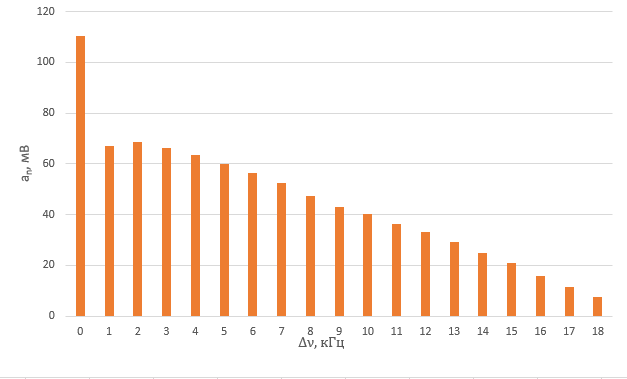
\includegraphics[width = 0.5\textwidth]			{Гармоники(1).png}}
	\subfloat[$f_\text{повт}$ = 1 кГц, $\tau$ = 			100 мкс]{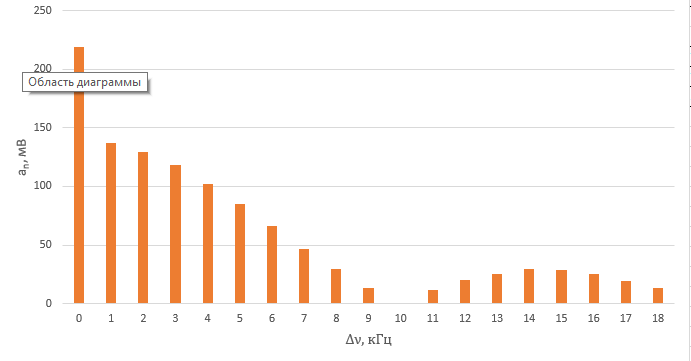
\includegraphics[width=0.5\textwidth]		{Гармоники(2).png}}
\caption{Вид спектра (прямоугольные импульсы)}
\end{figure}

\begin{figure}[h!]
\begin{center}
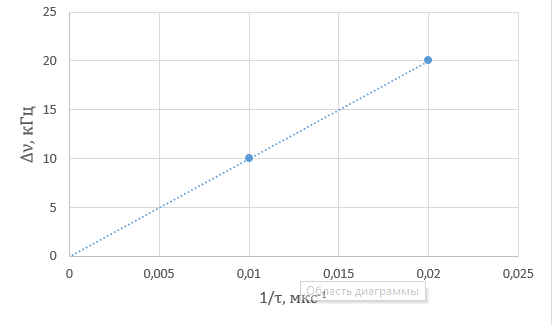
\includegraphics[scale=0.8]{nu(1t).png}
\end{center}
\caption{$\Delta \nu (1 \backslash \tau)$}
\label{nu(1/t)}
\end{figure}


Из графика \ref{nu(1/t)}:

\[k = \Delta \nu \tau = 1,\]

\noindentчто является частным случаем \textit{соотношения неопределенности} в квантовой механике.

\subsection*{Исследование спектра периодической последовательности цугов гармонических колебаний} 

Проанализируем, как меняется картина спектра при увеличении длительности $\tau$ импульса вдвое от 100 до 200 мкс ($f_\text{повт}$ = 1 кГц):

\begin{figure}[h!]
	\centering
	\subfloat[$\tau$ = 100 мкс]{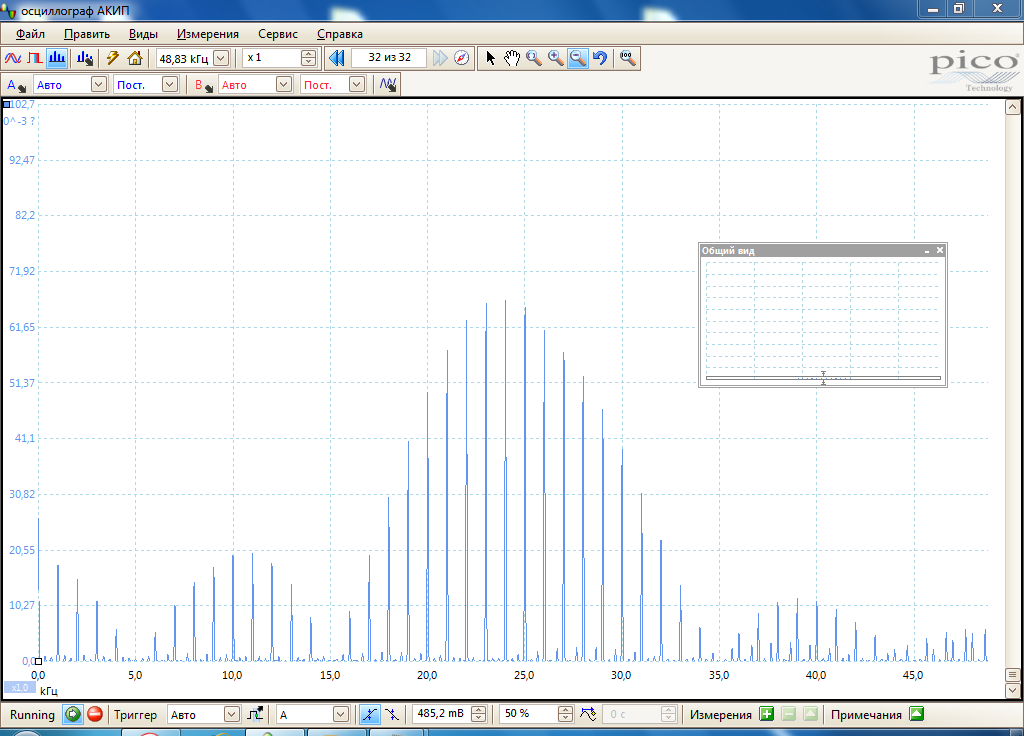
\includegraphics[width = 0.5\textwidth]				{100_tsugi.png}}
	\subfloat[$\tau$ = 200 мкс]						{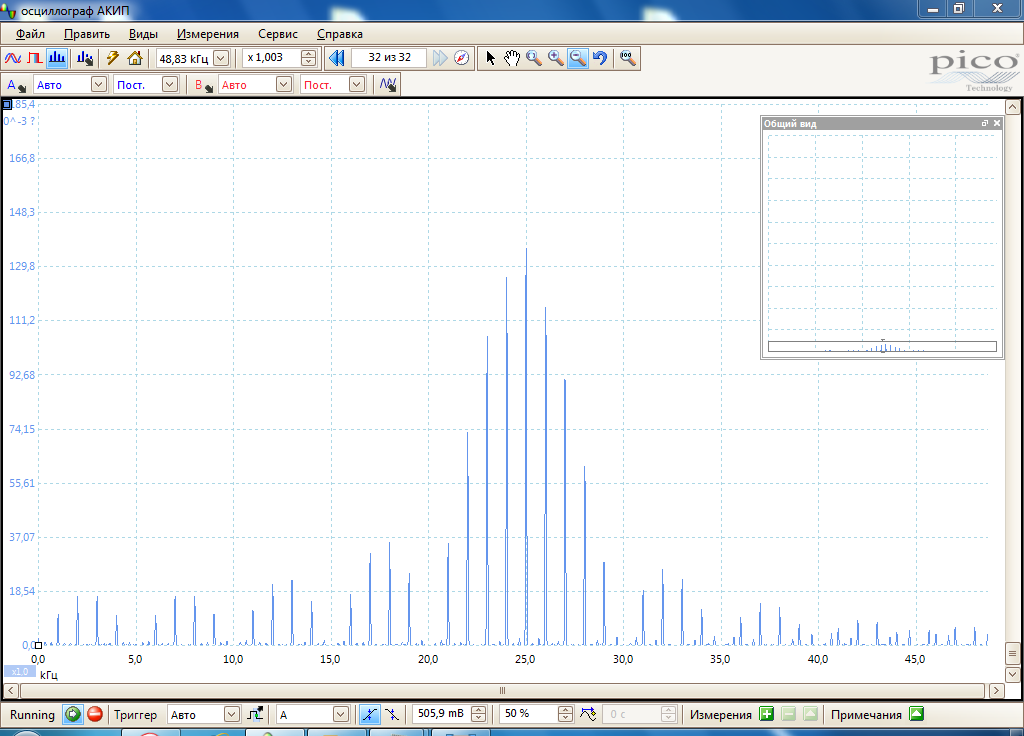
\includegraphics[width=0.5\textwidth]				{200_tsugi.png}}
\caption{Вид спектра (цуги)}
\end{figure}

Установим длительность импульса $\tau$ = 100 мкс, будем менять несущую частоту $\nu_0$ ($\nu_0$ = 10, 25, 40 кГц):

\begin{figure}[h!]
	\centering
	\subfloat[$\nu_0$ = 10 кГц]{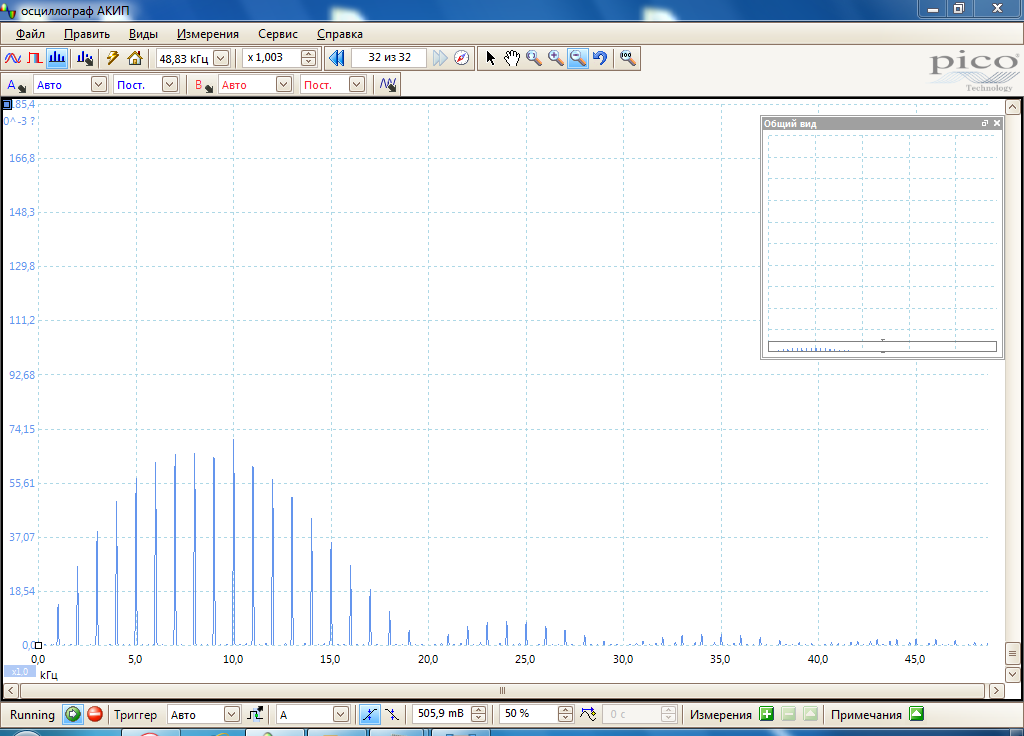
\includegraphics[width = 0.5\textwidth]				{nesuschaya_10.png}}
	\subfloat[$\nu_0$ = 25 кГц]						{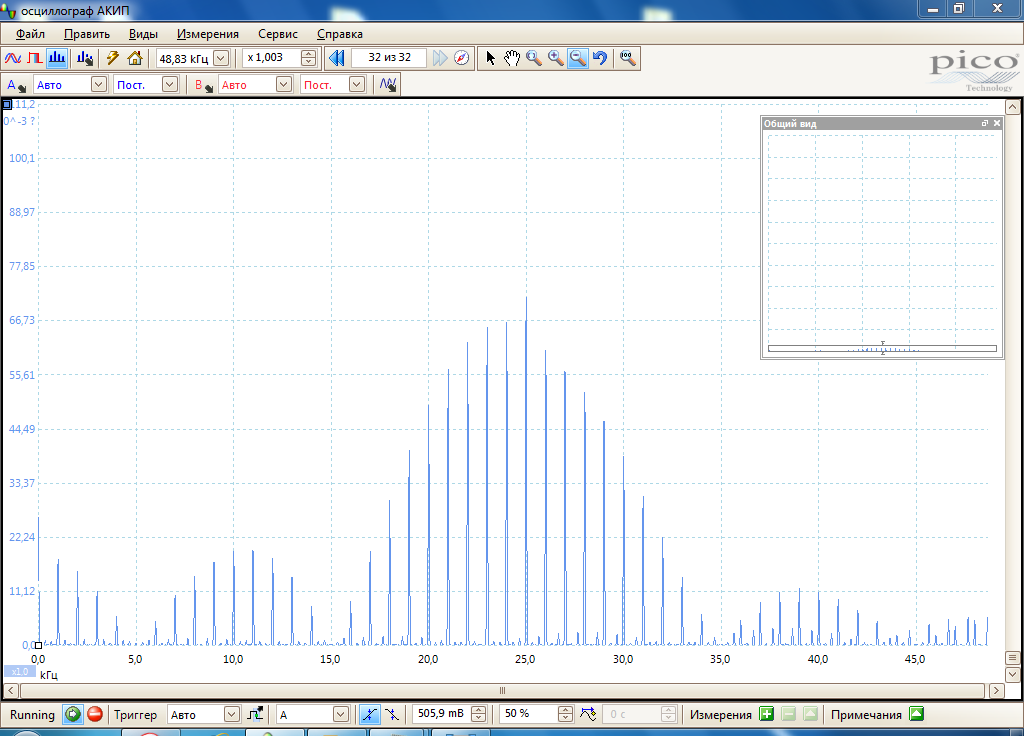
\includegraphics[width=0.5\textwidth]				{nesuschaya_25.png}}\\
	\subfloat[$\nu_0$ = 40 кГц]						{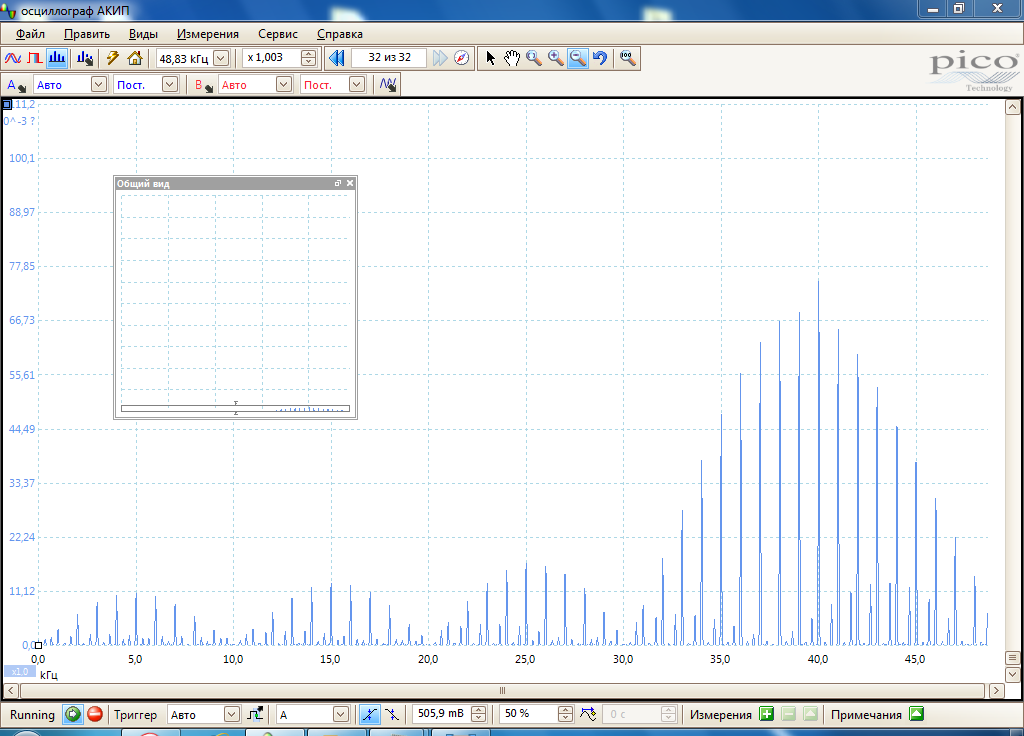
\includegraphics[width=0.5\textwidth]				{nesuschaya_40.png}}
\caption{Изменение несущей частоты $\nu_0$}
\end{figure}

\newpage
Установим несущую частоту $\nu_0$ = 30 кГц, длительность импульса $\tau$ = 100 мкс. Для разных частот повторения импульсов $f_\text{повт}$ определим расстояние $\delta \nu$:

\begin{table}[h!]
\centering
\caption{Зависимость $\delta \nu(f_\text{повт})$}
\begin{tabular}{|l|l|l|l|l|l|}
\hline
$f_\text{повт}$, кГц  & 0,5 & 1 & 2 & 4 & 5 \\ \hline
$\delta \nu$, кГц & 0,5 & 1 & 2 & 4 & 5 \\ \hline
\end{tabular}
\end{table}

\[\dfrac{\delta \nu}{f_\text{повт}} \approx 1\]

Установим $\tau$ = 100 мкс и $f_\text{повт}$ = 1 кГц, проведём измерения частот и амплитуд гармоник.


\end{document}